\subsubsection{UC3 - Login}
\begin{figure}[h]
	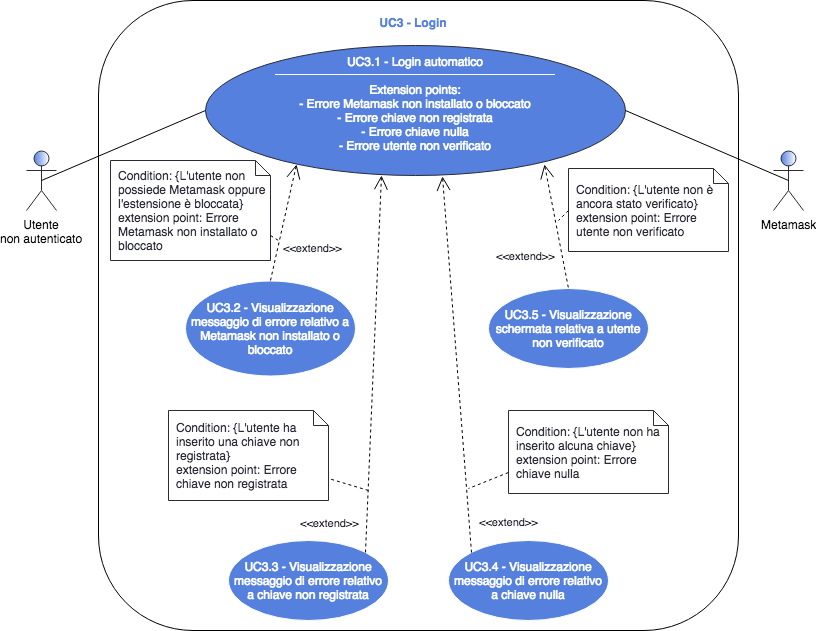
\includegraphics[width=10.5cm]{res/images/UC3Login.png} %da adattare in larghezza
	\centering
	\caption{UC3 - Login}
	
\end{figure}
\begin{itemize}
	\item \textbf{Attori Primari}:
	utente non autenticato;
	\item \textbf{Attori Secondari}:
	MetaMask\glosp;
	\item \textbf{Descrizione}:
	l'utente prova a farsi identificare tramite l'interfaccia web per mezzo di MetaMask\glosp;
	\item \textbf{Scenario}:
	l'utente non è identificato dal sito ed esegue il login;
	\item \textbf{Precondizione}:
	l'utente non è identificato dalla piattaforma web;
	\item \textbf{Postcondizione}:
	l'utente è identificato dalla piattaforma web. 
\end{itemize}
\subsubsection{UC3.1 - Login automatico}
\begin{itemize}
	\item \textbf{Attori Primari}:
	utente non autenticato;
	\item \textbf{Attori Secondari}:
	MetaMask\glosp;
	\item \textbf{Descrizione}:
	in modo automatico, il sistema procede all'identificazione dell'utente;
	\item \textbf{Scenario}:
	l'utente non ancora autenticato richiede il login;
	\item \textbf{Estensioni}:
	\begin{itemize}
		\item \textbf{UC2.5}: se l'utente non dispone di MetaMask\glosp o ha disabilitato l'estensione, viene visualizzato un messaggio di errore a riguardo;
		\item \textbf{UC2.6}: se l'utente non possiede una chiave\glosp su MetaMask\glo, esso viene avvisato tramite l'apposito messaggio di errore;
		\item \textbf{UC3.2}: se l'utente tenta di accedere al sito tramite MetaMask\glosp senza aver mai provveduto a registrarsi, riceverà un messaggio di errore a riguardo;
		
		\item \textbf{UC3.3}: se l'utente si è registrato sul sito da poco ma non gli è ancora stato validato l'account, visualizzerà un messaggio di errore a riguardo.
	\end{itemize}
	\item \textbf{Precondizione}:
	l'utente richiede alla piattaforma di venire identificato;
	\item \textbf{Postcondizione}:
	tramite il plugin MetaMask\glosp l'utente viene riconosciuto.
\end{itemize}
\subsubsection{UC3.2 - Visualizzazione messaggio di errore relativo a chiave non registrata}
\begin{itemize}
	\item \textbf{Attori Primari}:
	utente non autenticato;
	\item \textbf{Descrizione}:
	l'utente visualizza un messaggio di errore dovuto al fatto che ha tentato il login senza essersi registrato in precedenza;
	\item \textbf{Scenario}:
	l'utente tenta il login alla piattaforma senza aver effettuato la registrazione;
	\item \textbf{Precondizione}:
	l'utente richiede l'accesso al sito;
	\item \textbf{Postcondizione}:
	l'utente è consapevole di dover registrarsi per poter poi accedere.
\end{itemize}
\subsubsection{UC3.3 - Visualizzazione schermata relativa a utente non verificato}
\begin{itemize}
	\item \textbf{Attori Primari}:
	utente non autenticato;
	\item \textbf{Descrizione}:
	l'utente visualizza una schermata che esplica il fatto che il proprio account non è ancora stato verificato in seguito alla registrazione;
	\item \textbf{Scenario}:
	l'utente registrato da non molto tenta il login ma la richiesta viene rigettata, in quanto è a disposizione di un account non ancora validato;
	\item \textbf{Precondizione}:
	l'utente richiede il login alla piattaforma;
	\item \textbf{Postcondizione}: l'utente sa che dovrà attendere la validazione del propio account prima di procedere con il prossimo login.
\end{itemize}
\subsubsection{UC4 - Logout}
\begin{figure}[h]
	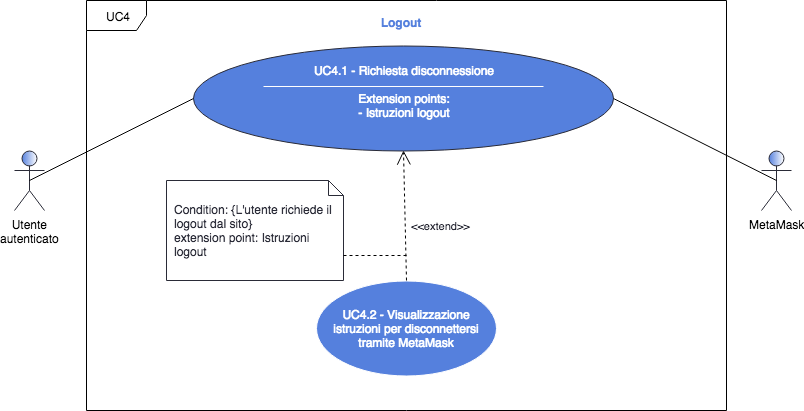
\includegraphics[width=15.5cm]{res/images/UC4Logout.png} %da adattare in larghezza
	\centering
	\caption{UC4 - Logout}
	
\end{figure}
\begin{itemize}
	\item \textbf{Attori Primari}:
	utente autenticato;
	\item \textbf{Attori Secondari}:
	MetaMask\glosp;
	\item \textbf{Descrizione}: l'utente richiede il logout dalla piattaforma web ed effettua ciò tramite MetaMask\glosp;
	\item \textbf{Scenario}: l'utente è identificato dal sito ed esegue il logout.
	\item \textbf{Precondizione}: l'utente è identificato dalla piattaforma web e richiede di essere disconnesso dal sito;
	\item \textbf{Postcondizione}: vengono fornite le istruzioni necessarie per affrontare il Logout tramite MetaMask\glosp. 
\end{itemize}
\subsubsection{UC4.1 - Richiesta disconnessione}
\begin{itemize}
	\item \textbf{Attori Primari}:
	utente autenticato;
	\item \textbf{Attori Secondari}:
	MetaMask\glosp;
	\item \textbf{Descrizione}: l'utente clicca sul bottone dedicato al logout e si appresta a leggere le istruzioni per farlo tramite MetaMask\glosp;
	\item \textbf{Scenario}: l'utente richiede la disconnessione dalla piattaforma web;
	\item \textbf{Inclusioni}:
	\begin{itemize}
		\item \textbf{UC4.2}: al conseguimento della richiesta di logout, l'utente riceve informazioni sul da farsi per procedere a completare ciò;
	\end{itemize}
	\item \textbf{Precondizione}: l'utente autenticato dal sistema non ha idea di come disconnettersi dal sito;
	\item \textbf{Postcondizione}: l'utente può visualizzare il modo corretto per eseguire la disconnessione dalla piattaforma.
	
\end{itemize}
\subsubsection{UC4.2 - Visualizzazione istruzioni per disconnettersi tramite MetaMask\glosp}
\begin{itemize}
	\item \textbf{Attori Primari}:
	utente autenticato;
	\item \textbf{Attori Secondari}:
	MetaMask\glosp;
	\item \textbf{Descrizione}: l'utente visualizza le istruzioni per procedere al logout tramite MetaMask\glosp;
	\item \textbf{Scenario}: in seguito alla richiesta di disconnessione, l'utente riceve le informazioni necessarie per effettuare tale operazione;
	
	\item \textbf{Precondizione}: l 'utente non ha idea di come disconnettersi tramite MetaMask\glo;
	\item \textbf{Postcondizione}: l'utente ha le abilità necessarie al conseguimento di un logout eseguito in modo corretto e sicuro tramite il plugin MetaMask\glo.
\end{itemize} 
